\documentclass{article}

% packages
  % basic stuff for rendering math
  \usepackage[letterpaper, top=1in, bottom=1in, left=1in, right=1in]{geometry}
  \usepackage[utf8]{inputenc}
  \usepackage[english]{babel}
  \usepackage{amsmath} 
  \usepackage{amssymb}
  % \usepackage{amsthm}

  % extra math symbols and utilities
  \usepackage{mathtools}        % for extra stuff like \coloneqq
  \usepackage{mathrsfs}         % for extra stuff like \mathsrc{}
  \usepackage{centernot}        % for the centernot arrow 
  \usepackage{bm}               % for better boldsymbol/mathbf 
  \usepackage{enumitem}         % better control over enumerate, itemize
  \usepackage{hyperref}         % for hypertext linking
  \usepackage{fancyvrb}          % for better verbatim environments
  \usepackage{newverbs}         % for texttt{}
  \usepackage{xcolor}           % for colored text 
  \usepackage{listings}         % to include code
  \usepackage{lstautogobble}    % helper package for code
  \usepackage{parcolumns}       % for side by side columns for two column code
  

  % page layout
  \usepackage{fancyhdr}         % for headers and footers 
  \usepackage{lastpage}         % to include last page number in footer 
  \usepackage{parskip}          % for no indentation and space between paragraphs    
  \usepackage[T1]{fontenc}      % to include \textbackslash
  \usepackage{footnote}
  \usepackage{etoolbox}

  % for custom environments
  \usepackage{tcolorbox}        % for better colored boxes in custom environments
  \tcbuselibrary{breakable}     % to allow tcolorboxes to break across pages

  % figures
  \usepackage{pgfplots}
  \pgfplotsset{compat=1.18}
  \usepackage{float}            % for [H] figure placement
  \usepackage{tikz}
  \usepackage{tikz-cd}
  \usepackage{circuitikz}
  \usetikzlibrary{arrows}
  \usetikzlibrary{positioning}
  \usetikzlibrary{calc}
  \usepackage{graphicx}
  \usepackage{caption} 
  \usepackage{subcaption}
  \captionsetup{font=small}

  % for tabular stuff 
  \usepackage{dcolumn}

  \usepackage[nottoc]{tocbibind}
  \pdfsuppresswarningpagegroup=1
  \hfuzz=5.002pt                % ignore overfull hbox badness warnings below this limit

% New and replaced operators
  \DeclareMathOperator{\Tr}{Tr}
  \DeclareMathOperator{\Sym}{Sym}
  \DeclareMathOperator{\Span}{span}
  \DeclareMathOperator{\std}{std}
  \DeclareMathOperator{\Cov}{Cov}
  \DeclareMathOperator{\Var}{Var}
  \DeclareMathOperator{\Corr}{Corr}
  \DeclareMathOperator{\pos}{pos}
  \DeclareMathOperator*{\argmin}{\arg\!\min}
  \DeclareMathOperator*{\argmax}{\arg\!\max}
  \newcommand{\ket}[1]{\ensuremath{\left|#1\right\rangle}}
  \newcommand{\bra}[1]{\ensuremath{\left\langle#1\right|}}
  \newcommand{\braket}[2]{\langle #1 | #2 \rangle}
  \newcommand{\qed}{\hfill$\blacksquare$}     % I like QED squares to be black

% Custom Environments
  \newtcolorbox[auto counter, number within=section]{question}[1][]
  {
    colframe = orange!25,
    colback  = orange!10,
    coltitle = orange!20!black,  
    breakable, 
    title = \textbf{Question \thetcbcounter ~(#1)}
  }

  \newtcolorbox[auto counter, number within=section]{exercise}[1][]
  {
    colframe = teal!25,
    colback  = teal!10,
    coltitle = teal!20!black,  
    breakable, 
    title = \textbf{Exercise \thetcbcounter ~(#1)}
  }
  \newtcolorbox[auto counter, number within=section]{solution}[1][]
  {
    colframe = violet!25,
    colback  = violet!10,
    coltitle = violet!20!black,  
    breakable, 
    title = \textbf{Solution \thetcbcounter}
  }
  \newtcolorbox[auto counter, number within=section]{lemma}[1][]
  {
    colframe = red!25,
    colback  = red!10,
    coltitle = red!20!black,  
    breakable, 
    title = \textbf{Lemma \thetcbcounter ~(#1)}
  }
  \newtcolorbox[auto counter, number within=section]{theorem}[1][]
  {
    colframe = red!25,
    colback  = red!10,
    coltitle = red!20!black,  
    breakable, 
    title = \textbf{Theorem \thetcbcounter ~(#1)}
  } 
  \newtcolorbox[auto counter, number within=section]{proposition}[1][]
  {
    colframe = red!25,
    colback  = red!10,
    coltitle = red!20!black,  
    breakable, 
    title = \textbf{Proposition \thetcbcounter ~(#1)}
  } 
  \newtcolorbox[auto counter, number within=section]{corollary}[1][]
  {
    colframe = red!25,
    colback  = red!10,
    coltitle = red!20!black,  
    breakable, 
    title = \textbf{Corollary \thetcbcounter ~(#1)}
  } 
  \newtcolorbox[auto counter, number within=section]{proof}[1][]
  {
    colframe = orange!25,
    colback  = orange!10,
    coltitle = orange!20!black,  
    breakable, 
    title = \textbf{Proof. }
  } 
  \newtcolorbox[auto counter, number within=section]{definition}[1][]
  {
    colframe = yellow!25,
    colback  = yellow!10,
    coltitle = yellow!20!black,  
    breakable, 
    title = \textbf{Definition \thetcbcounter ~(#1)}
  } 
  \newtcolorbox[auto counter, number within=section]{example}[1][]
  {
    colframe = blue!25,
    colback  = blue!10,
    coltitle = blue!20!black,  
    breakable, 
    title = \textbf{Example \thetcbcounter ~(#1)}
  } 
  \newtcolorbox[auto counter, number within=section]{code}[1][]
  {
    colframe = green!25,
    colback  = green!10,
    coltitle = green!20!black,  
    breakable, 
    title = \textbf{Code \thetcbcounter ~(#1)}
  } 

  \BeforeBeginEnvironment{example}{\savenotes}
  \AfterEndEnvironment{example}{\spewnotes}
  \BeforeBeginEnvironment{lemma}{\savenotes}
  \AfterEndEnvironment{lemma}{\spewnotes}
  \BeforeBeginEnvironment{theorem}{\savenotes}
  \AfterEndEnvironment{theorem}{\spewnotes}
  \BeforeBeginEnvironment{corollary}{\savenotes}
  \AfterEndEnvironment{corollary}{\spewnotes}
  \BeforeBeginEnvironment{proposition}{\savenotes}
  \AfterEndEnvironment{proposition}{\spewnotes}
  \BeforeBeginEnvironment{definition}{\savenotes}
  \AfterEndEnvironment{definition}{\spewnotes}
  \BeforeBeginEnvironment{exercise}{\savenotes}
  \AfterEndEnvironment{exercise}{\spewnotes}
  \BeforeBeginEnvironment{proof}{\savenotes}
  \AfterEndEnvironment{proof}{\spewnotes}
  \BeforeBeginEnvironment{solution}{\savenotes}
  \AfterEndEnvironment{solution}{\spewnotes}
  \BeforeBeginEnvironment{question}{\savenotes}
  \AfterEndEnvironment{question}{\spewnotes}
  \BeforeBeginEnvironment{code}{\savenotes}
  \AfterEndEnvironment{code}{\spewnotes}

  \definecolor{dkgreen}{rgb}{0,0.6,0}
  \definecolor{gray}{rgb}{0.5,0.5,0.5}
  \definecolor{mauve}{rgb}{0.58,0,0.82}
  \definecolor{lightgray}{gray}{0.93}

  % default options for listings (for code)
  \lstset{
    autogobble,
    frame=ltbr,
    language=C,                           % the language of the code
    aboveskip=3mm,
    belowskip=3mm,
    showstringspaces=false,
    columns=fullflexible,
    keepspaces=true,
    basicstyle={\small\ttfamily},
    numbers=left,
    firstnumber=1,                        % start line number at 1
    numberstyle=\tiny\color{gray},
    keywordstyle=\color{blue},
    commentstyle=\color{dkgreen},
    stringstyle=\color{mauve},
    backgroundcolor=\color{lightgray}, 
    breaklines=true,                      % break lines
    breakatwhitespace=true,
    tabsize=3, 
    xleftmargin=2em, 
    framexleftmargin=1.5em, 
    stepnumber=1
  }

% Page style
  \pagestyle{fancy}
  \fancyhead[L]{Algorithms}
  \fancyhead[C]{Muchang Bahng}
  \fancyhead[R]{Spring 2024} 
  \fancyfoot[C]{\thepage / \pageref{LastPage}}
  \renewcommand{\footrulewidth}{0.4pt}          % the footer line should be 0.4pt wide
  \renewcommand{\thispagestyle}[1]{}  % needed to include headers in title page

\begin{document}

\title{Algorithms}
\author{Muchang Bahng}
\date{Spring 2024}

\maketitle
\tableofcontents
\pagebreak

\section{Complexity}

    A course on the study of algorithms. 

    \begin{definition}[Algorithm]
      An \textbf{algorithm} is a procedure for solving a mathematical problem in a \textit{finite} number of steps. It should be 
      \begin{enumerate}
        \item finite, 
        \item correct,
        \item efficient
      \end{enumerate}
    \end{definition}

    An algorithm, with respect to some inputs $\mathbf{n}$, will have a runtime that is some function $f$. We would like a formal way to analyze the asymptotic behavior between two functions. 

    \begin{definition}[Complexity]
      Given two positive functions $f, g$, 
      \begin{enumerate}
        \item $f = O(g)$ if $f/g$ is bounded.\footnote{Note that it is more accurate to write $f \in O(g)$, since we consider $O(g)$ a class of functions for which the property holds.} 
        \item $f = \Omega(g)$ if $g/f$ is bounded, i.e. $g = O(f)$. 
        \item $f = \Theta (g)$ if $f = O(g)$ and $g = O(f)$. 
      \end{enumerate}
    \end{definition}

    There are two notions of complexity here. We can compare $f$ and $g$ with respect to the \textit{value} $N$ of the input, or we can compare them with respect to the \textit{number of bits} $n$ in the input. While we mostly use the complexity w.r.t. the value, we should be aware for certain (especially low-level operations), the bit complexity is also important. 

    Let's do a quick comparison of various functions. Essentially, if we want to figure out the complexity of two positive functions $f, g$,\footnote{These will be positive since the runtime must be positive.} we can simply take the limit. 
    \begin{equation}
      \lim_{x \rightarrow +\infty} \frac{f(x)}{g(x)} = \begin{cases} 
        0 & \implies f = O(g) \\
        0 < x < +\infty & \implies f = \Theta(g) \\
        +\infty & \implies f = \Omega(g)
      \end{cases}
    \end{equation} 

    Most of the time, we will have to use L'Hopital's rule to derive these actual limits, but the general trend is 
    \begin{enumerate}
      \item $\log n$ is small  
      \item $\mathrm{poly}(n)$ grows faster
      \item $\exp(n)$ grows even faster 
      \item $n!$ even faster
      \item $n^n$ even faster
    \end{enumerate}

    \begin{theorem}[Properties]
      Some basic properties, which shows very similar properties to a vector space. 
      \begin{enumerate}
        \item Transitivity. 
        \begin{align}
          f = O(g), g = O(h) & \implies f = O(h) \\
          f = \Omega(g), g = \Omega(h) & \implies f = \Omega(h) \\
          f = \Theta(g), g = \Theta(h) & \implies f = \Theta(h) \\
        \end{align}

        \item Linearity.  
          \begin{align}
            f = O(h), g = O(h) & \implies f + g = O(h) \\
            f = \Omega(h), g = \Omega(h) & \implies f + g = \Omega(h) \\
            f = \Theta(h), g = \Theta(h) & \implies f + g = \Theta(h) \\
          \end{align}
      \end{enumerate}
    \end{theorem}

    \begin{example}
      Compare the following functions. 
      \begin{enumerate}
        \item $f(n) = \log_{10} (n), g(n) = \log_2 (n)$. Since they are different bases, we can write $f(n) = \log (n) / \log (10)$ and $g(n) = \log(n) / \log(2)$. They differ by a constant factor, so $f = \Theta(g)$. 

        \item $f(n) = (\log n)^{20}, g(n) = n$. We have 
        \begin{equation}
          \lim_{n \rightarrow \infty} \frac{(\log n)^20}{n} = \lim_{n \rightarrow \infty} \frac{20 \cdot (\log n)^{19} \cdot \frac{1}{n}}{1} = \ldots = \lim_{n \rightarrow \infty} \frac{20!}{n} = 0 \implies f = O(g)
        \end{equation}

        \item $f(n) = n^{100}, g(n) = 1.01^n$. We have 
          \begin{equation}
            \lim_{n \rightarrow \infty} \frac{n^{100}}{1.01^n} = \lim_{n \rightarrow \infty} \frac{100 n^{99}}{1.01^n \cdot \log (1.01)} =  \ldots = \lim_{n \rightarrow \infty} \frac{100!}{1.01^n \cdot (\log 1.01)^100} = 0 \implies f = O(g)
          \end{equation}
      \end{enumerate}
    \end{example}

    Let's do a slightly more nontrivial example. 

    \begin{example}
      Given the following algorithm, what is the runtime? 
      \begin{lstlisting}
        for i in range(1, n+1): 
          j = 1 
          while j <= i: 
            j = 2 * j
      \end{lstlisting}
      Now we can see that for each $i$, we will double up to $\log_2 (i)$ times. Therefore summing this all over $i$ is 
      \begin{equation}
        \sum_{i = 1}^n \log_2 (i) = \log_2 (n!) \leq \log_2 (n^n) = n \log_2 (n)
      \end{equation}
      and so we can see that the runtime is $O(n \log n)$. Other ways to do this is to just replace the summation with an integral.\footnote{Need more justification on why this is the case. Mentioned in lecture.} 
      \begin{equation}
        \int_1^n \log_2 (x) \,dx = x \log(x) - x \big|_1^n = n \log(n) - n + 1 = O(n \log n)
      \end{equation}
    \end{example}

  \subsection{Recursive Algorithms and Recurrence Relation}

    I assume that the reader is familiar with recursive algorithms. Now to evaluate the runtime of a recursive algorithm, one must implicitly solve for the runtime of its recursive calls. 

\section{Brute Force Algorithms} 

  \subsection{Basic Arithmetic}

    In here, we use basic deductions from elementary algebra to give us a starting point at which we analyze fundamental arithmetic algorithms. 

    \begin{theorem}[Complexity of Addition]
      The complexity of addition of two $O(N)$ values with $n$ bits is
      \begin{enumerate}
        \item $O(n)$ bit complexity. 
        \item $O(\log N)$ complexity. 
        \item $O(1)$ memory complexity. 
      \end{enumerate}
      By the same logic, the complexity of subtraction is 
      \begin{enumerate}
        \item $O(n)$ bit complexity. 
        \item $O(\log N)$ complexity. 
        \item $O(1)$ memory complexity. 
      \end{enumerate}
    \end{theorem}
    \begin{proof}
      To see bit complexity, we are really taking each bit of each number and adding them together, plus a potential carry operation. Therefore, we are doing a bounded number of computations per bit, which is $O(1)$, but we must at least read through all of the bits, making this $O(\max\{n, m\})$. 
    \end{proof}

    \begin{theorem}[Complexity of Multiplication]
      The complexity of multiplication of two values $N, M$ with bits $n, m$ is 
      \begin{enumerate}
        \item $O(n^2)$ bit complexity.\footnote{It turns out we can do better, which we will learn later.} 
        \item $O((\log n)^2)$ complexity. 
        \item 
      \end{enumerate}
    \end{theorem}

    \begin{theorem}[Complexity of Division]
      The complexity of multiplication of two values $N, M$ with bits $n, m$ is 
      \begin{enumerate}
        \item $O(n^2)$ bit complexity. 
        \item 
      \end{enumerate}
    \end{theorem}

    \begin{theorem}[Complexity of Modulus]
      The complexity of multiplication of two values $N, M$ with bits $n, m$ is 
      \begin{enumerate}
        \item $O(n^2)$ bit complexity. 
        \item 
      \end{enumerate}
    \end{theorem}

    \begin{theorem}[Complexity of Exponentiation]
      The complexity of multiplication of two values $N, M$ with bits $n, m$ is 
      \begin{enumerate}
        \item $O(n^2)$ bit complexity. 
        \item 
      \end{enumerate}
    \end{theorem}

    \begin{theorem}[Complexity of Square Root]
      The complexity of multiplication of two values $N, M$ with bits $n, m$ is 
      \begin{enumerate}
        \item $O(n^2)$ bit complexity. 
        \item 
      \end{enumerate}
    \end{theorem}

    \begin{definition}[Factorial]
      
    \end{definition}
  
  \subsection{Lists} 

    \begin{definition}[Max and Min of List]
      
    \end{definition}

    \begin{definition}[Bubble Sort]

    \end{definition}

    \begin{definition}[Binary Search]
      
    \end{definition}

  \subsection{Cryptography} 

    \begin{example}[GCD of Two Numbers]
      Take a look at the following algorithm. 
      \begin{lstlisting}
        def gcd(a, b): 
          if a == b: 
            return a
          elif a > b: 
            return gcd(a - b, b) 
          else: 
            return gcd(a, b - a)

        print(gcd(63, 210))
      \end{lstlisting}
    \end{example}

    \begin{definition}[Primality Testing]
      
    \end{definition}

    \begin{definition}[Integer Factorization]
      
    \end{definition}

  \subsection{Matrix Operations}

    \begin{definition}[Matrix Multiplication]
      
    \end{definition}

    \begin{definition}[Singular Value Decomposition]
      
    \end{definition}

    \begin{definition}[QR Decomposition]
      
    \end{definition}

    \begin{definition}[LU Decomposition]
      
    \end{definition}

    \begin{definition}[Matrix Inversion]
      
    \end{definition}

\section{Divide and Conquer} 

  \begin{definition}[Divide and Conquer Algorithms]
    
  \end{definition}

  \subsection{Karatsuba Algorithm for Multiplication}

  \subsection{Merge Sort}

  \subsection{Strassen Algorithm}

  \subsection{Fast Fourier Transform}

\section{Hashing and Probabilistic Algorithms}

  \subsection{Modulo Operations}
  
  \subsection{Hashing}

  \subsection{Primality Testing}

\section{Dynamic Programming}

  \subsection{Longest Increasing Subsequence}

  \subsection{Knapsack}

\section{Graphs}

    A huge portion of problems can be solved by representing as a \textit{graph} data structure. In here, we will explore various problems that can be solved through \textit{graph algorithms}. 

  \subsection{Representations and Properties}

    All graphs consist of a set of vertices/nodes $V$ and edges $E$. This tuple is what makes up a graph. We denote $|V| = n, |E| = m$. 

    \begin{definition}[Undirected Graphs]
      An \textbf{undirected graph} $G(V, E)$ is a tuple, where $V = \{v_1, \ldots, v_n\}$ is the vertex set and $E = \{\{v_i, v_j\}\}$ is the edge set (note that it is a set of sets!). 
      \begin{enumerate}
        \item The \textbf{degree} $d_v$ of a vertex $v$ is the number of edges incident to it. 
        \item A \textbf{path} is a sequence of vertices where adjacent vertices are connected by a path in $E$. It's \textbf{length} is the number of edges in the path. 
        \item A \textbf{cycle} is a path that has the same start and end. 
        \item A graph is \textbf{connected} if for every pair of vertices $e_i, e_j \in E$, there is a path from 
        \item A \textbf{connected component} is a maximal subset of connected vertices. 
      \end{enumerate}
    \end{definition}

    \begin{definition}[Directed Graph]
      A \textbf{directed graph} $G(V, E)$ is a tuple, where $V = \{v_1, \ldots, v_n\}$ is the vertex set and $E = \{(v_i, v_j)\}$ is the edge set (note that it is a set of tuples, so $(i, j) \neq ( j, i)$).
      \begin{enumerate}
        \item The \textbf{in/out degree} $d_{v, i}, d_{v, o}$ of a vertex $v$ is the number of edges going in to or out from $v$. 
        \item 
      \end{enumerate}
    \end{definition}

    In fact, from these definitions alone, we can solve an ancient puzzle called \textit{the Bridges of Konigsberg}. Euler, in trying to solve this problem, had invented graph theory. 

    \begin{example}[Bridges of Konigsberg]
      Is there a way to walk that crosses each bridge \textit{exactly} once? 
      \begin{figure}[H]
        \centering 
        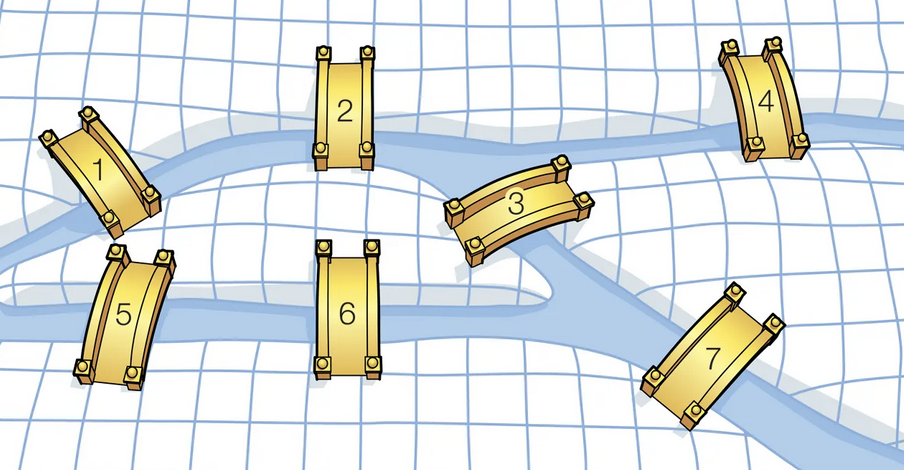
\includegraphics[scale=0.4]{img/bridges.png}
        \caption{Bridges of Konigsberg} 
        \label{fig:bridges}
      \end{figure}
      It can be decomposed into this undirected graph. 
      \begin{figure}[H]
        \centering 
        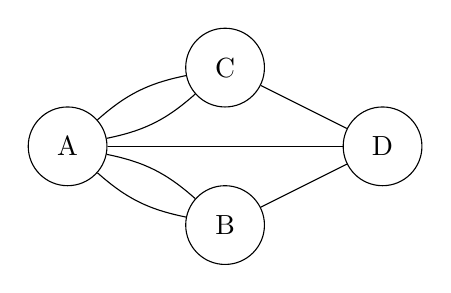
\begin{tikzpicture} 
          \tikzstyle{every node}=[circle, draw, minimum size=1cm]
          
          \node (A) at (0,0) {A};
          \node (B) at (2,-1) {B};
          \node (C) at (2,1) {C};
          \node (D) at (4,0) {D}; 
                
          \draw (A) to[bend left=15] (B);
          \draw (A) to[bend right=15] (B);
          \draw (A) to[bend left=15] (C);
          \draw (A) to[bend right=15] (C);
          \draw (A) -- (D);
          \draw (B) -- (D);
          \draw (C) -- (D);
        \end{tikzpicture}
        \caption{Graph representation. } 
        \label{fig:bridge_graph}
      \end{figure}
      Euler's observation is that except for start and end points, a talk leaves any vertex by different edge that the incoming edge. Therefore, the degree (number of edges incident on it) must have an even number, so all but 2 vertices must have an even degree. Since every vertex has an odd degree, there is no way of doing it. 
    \end{example}

    In addition to the \textit{adjacency list} representation, another way in which we represent a directed graph is through \textit{adjacency matrices}. 

    \begin{definition}[Adjacency Matrix]
      In a finite directed graph $(V, E)$, we can construct a bijection from $V$ to the natural numbers and so we label each element in $V$ with $i \in \mathbb{N}$. Then, we can construct a matrix $A$ such that 
      \begin{equation}
        A_{ij} = \begin{cases} 1 & \text{ if } (i, j) \in E \\ 0 & \text{ if } (i, j) \not\in E \end{cases}
      \end{equation}
    \end{definition}

    While the adjacency matrix does have its advantages and has a cleaner form, usually in sparse graphs this is memory inefficient due to there being an overwhelming number of $0$s. 

    \begin{definition}[Trees]
      An undirected graph $G(V, E)$ is a \textbf{tree} if 
      \begin{enumerate}
        \item $G$ is connected. 
        \item $G$ has no cycles.\footnote{This makes sense, since to get back to a previous vertex you must backtrack.}
      \end{enumerate}
      Removing the first requirement gives us the definition of a \textbf{forest}, which is a collection of trees. Conversely, if $G(V, E)$ is connected  and $|E| = n - 1$, then $G$ is a tree. 
    \end{definition}

    \begin{theorem}[Properties of Trees]
      If $G(V, E)$ is a tree, then 
      \begin{enumerate}
        \item There exists a $v \in V$ s.t. $d_v = 1$, called a \textbf{leaf node}. 
        \item $|E| = |V| - 1 = n - 1$. 
      \end{enumerate}
    \end{theorem}
    \begin{proof}
      The outlines are quite intuitive. 
      \begin{enumerate}
        \item There must be some leaf node since if there wasn't, then we would have a cycle. We can use proof by contradiction. 
        \item We can use proof by induction. We start off with one vertex and to construct a tree, we must add one edge and one vertex at every step, keeping this invariant.  
      \end{enumerate}
    \end{proof}

  \subsection{Exploration}

    Given two $v, s \in V$ either directed or undirected, how can we find the shortest path from $v$ to $s$? 

    \begin{definition}[Depth First Search]
      
    \end{definition}

    \begin{theorem}[Runtime of DFS]
      
    \end{theorem}

    \begin{definition}[Breath First Search]
      
    \end{definition}

    This can be used to make a \textit{BFS tree}. 

    \begin{definition}[BFS Tree]
      
    \end{definition}

    \begin{theorem}[Runtime of BFS]
      To get the running time, we know that each vertex is popped only once from the queue, giving us $O(n)$. For each pop, we are exploring all the neighbors of $V$. 
      \begin{align}
        O \bigg( \sum_{v \in V} | \text{neighbors of } v| + 1\bigg) & = O \bigg( \sum_{v \in V} d_v + 1 \bigg) \\
                                             & = O (2 |E| + |V|) = O(m + n )
      \end{align}
      which is linear in input size!  
    \end{theorem}

    \begin{exercise}
      Prove that in any connected undirected graph $G = (V, E)$ there is a vertex $v \in V$ s.t. $G$ remains connected after removing $v$. 
    \end{exercise}
    \begin{proof}
      You can make a BFS tree from this graph, and there has to be a last layer. Just remove the node from this layer. 
    \end{proof}

    \begin{exercise}
      Give an example of a strongly connected directed graph $G = (V, E)$ s.t. that every $v \in V$, removing $v$ from $G$ gives a directed graph that is not strongly connected. 
    \end{exercise}
    
    \begin{exercise}[DPV 3.16]
    \end{exercise}
    \begin{proof}
      Do BFS but now recursively store the maximum of all the prerequisite courses plus 1 for the current course. 
    \end{proof}

  \subsection{Bipartite Graphs}

    \begin{definition}[Bipartite Graph]
      A \textbf{bipartite graph} is an undirected graph $G(V, L)$ where we can partition $V = L \sqcup R$ such that for all $e = \{u, v\} \in E$, we have $u \in L, v \in R$.  
    \end{definition}

    We would like to devise some method to determine if an arbitrary graph is bipartite. 

    \begin{theorem}
      $G$ is bipartite if and only if all cycles in $G$ are even length. 
    \end{theorem}
    \begin{proof}
      Proving $(\implies)$ is quite easy since if we suppose $G$ has an odd length cycle, then we start packing vertices of a cycle into $L, R$, but by the time we came back to the start, we are forced to pack it into the wrong partition! 

      The converse is quite hard to prove, and we'll take it at face value. 
    \end{proof}

    \begin{example}[Determine Bipartite]
      Given an arbitrary graph, I want to determine if it is bipartite. 
      \begin{enumerate}
        \item We first run BFS on the graph starting at $s \in V$, which divides it up into layers representing the shortest path from $s$. 
        \item Then for each layer $L_i \subset V$, we check if there are connections between two vertices $x, y \in L_i$. If there are connections, then this is not bipartite. If there are none, then this is bipartite. 
      \end{enumerate}
    \end{example}

\section{Approximation Algorithms}

  \subsection{Greedy Algorithms}

\section{Linear Programming}

\end{document}
